\documentclass[10pt,a4paper]{article}

% -----------------------------------------------------------------------------
% MATHS MANTHAN | Class 10 Triangles Handbook | Academic Year 2026--27
% Publication-Quality Formula & Concept Master Handbook for CBSE Class 10
% Fully compliant with rationalized CBSE 2026--27 curriculum (Chapter 6: Triangles)
% Compile with pdfLaTeX twice to resolve LastPage and cross-references.
% -----------------------------------------------------------------------------

\usepackage[a4paper,top=12mm,bottom=16mm,left=15mm,right=15mm,footskip=8mm]{geometry}
\usepackage[T1]{fontenc}
\usepackage{lmodern}
\usepackage{microtype}
\usepackage{amsmath,amssymb}
\usepackage[table]{xcolor}
\usepackage{array,tabularx,booktabs}
\usepackage{graphicx}
\usepackage{eso-pic}
\usepackage{tikz}
\usetikzlibrary{calc,positioning,arrows.meta,shapes.geometric,patterns}
\usepackage[most]{tcolorbox}
\usepackage{enumitem}
\usepackage{fancyhdr}
\usepackage{lastpage}
\usepackage[hidelinks]{hyperref}
\usepackage{url}

% Compatibility fix for colortbl + tabularx p-column alignment
\makeatletter
\let\insert@pcolumn\insert@column
\makeatother

% ============================================================================
% BRAND COLOR PALETTE — 100% UNIFORM WITH MATHS MANTHAN STANDARDS
% Primary Navy: #001F49 | Brand Gold: #D19029 | Secondary Slate: #4B5563
% ============================================================================
\definecolor{primary}{RGB}{0,31,73}
\definecolor{brandnavy}{RGB}{0,31,73}
\definecolor{accent}{RGB}{209,144,41}
\definecolor{brandgold}{RGB}{209,144,41}
\definecolor{secondary}{RGB}{75,85,99}
\definecolor{lightgray}{RGB}{246,248,250}
\definecolor{accentlight}{RGB}{254,250,242}
\definecolor{primarylight}{RGB}{240,244,250}

\colorlet{navy}{primary}
\colorlet{blue}{primary!82!black}
\colorlet{gold}{accent}
\colorlet{goldpale}{accentlight}
\colorlet{bluepale}{primarylight}
\colorlet{ink}{secondary}
\colorlet{muted}{secondary}
\colorlet{linegray}{primary!25}
\colorlet{reddeep}{primary}
\colorlet{redpale}{lightgray}
\colorlet{green}{primary}
\colorlet{greenpale}{primarylight}

% Automatic low-opacity logo watermark on every page
\IfFileExists{mathsmanthan logo.png}{%
  \AddToShipoutPictureBG{%
    \begin{tikzpicture}[remember picture,overlay]
      \node[opacity=0.065] at (current page.center) {%
        \includegraphics[width=0.55\paperwidth,keepaspectratio]{mathsmanthan logo.png}%
      };
    \end{tikzpicture}%
  }%
}{}

\hypersetup{
  pdftitle={Class 10 Triangles | Maths Manthan Master Handbook},
  pdfauthor={Maths Manthan Tuition Classes},
  pdfsubject={CBSE Class 10 Mathematics, Academic Year 2026--27},
  pdfkeywords={Triangles, Similarity, BPT, Thales Theorem, Class 10, CBSE, Geometry, Maths Manthan, Formula Handbook, 2026-27}
}

\setlength{\parindent}{0pt}
\setlength{\parskip}{2.2pt}
\renewcommand{\arraystretch}{1.14}
\setlist[itemize]{leftmargin=5mm,itemsep=1.2pt,topsep=1.2pt,parsep=0pt}
\setlist[enumerate]{leftmargin=5.5mm,itemsep=1.2pt,topsep=1.2pt,parsep=0pt}
\setlength{\tabcolsep}{4.5pt}
\emergencystretch=2em
\hfuzz=1pt

% ============================================================================
% HEADER / FOOTER SPECIFICATION
% ============================================================================
\newcommand{\TuitionName}{{\color{primary}MATHS} {\color{accent}MANTHAN}}
\newcommand{\TuitionSub}{{\color{primary}\textbullet\ \ \text{TUITION CLASSES}\ \ \textbullet}}
\newcommand{\ContactInfo}{e-mail: contact@mathsmanthan.co.in \quad$\vert$\quad Helpline: +91-8171546558}
\newcommand{\HandbookFooterTitle}{Class 10 Triangles Handbook}

\pagestyle{fancy}
\fancyhf{}
\renewcommand{\headrulewidth}{0pt}
\renewcommand{\footrulewidth}{0.6pt}
\renewcommand{\footrule}{\hbox to\headwidth{\color{primary!30}\leaders\hrule height 0.6pt\hfill}}
\fancyfoot[L]{\footnotesize\href{https://mathsmanthan.co.in}{\textcolor{secondary}{\TuitionName\ $\vert$\ \HandbookFooterTitle}}}
\fancyfoot[R]{\footnotesize\textbf{\color{primary}Page \thepage\ of \pageref{LastPage}}\quad\textcolor{accent}{\textbf{Academic Year 2026--27}}}

\fancypagestyle{plain}{%
  \fancyhf{}
  \fancyfoot[L]{\footnotesize\href{https://mathsmanthan.co.in}{\textcolor{secondary}{\TuitionName\ $\vert$\ \HandbookFooterTitle}}}
  \fancyfoot[R]{\footnotesize\textbf{\color{primary}Page \thepage\ of \pageref{LastPage}}\quad\textcolor{accent}{\textbf{Academic Year 2026--27}}}
  \renewcommand{\headrulewidth}{0pt}
  \renewcommand{\footrulewidth}{0.6pt}
  \renewcommand{\footrule}{\hbox to\headwidth{\color{primary!30}\leaders\hrule height 0.6pt\hfill}}
}

% Institutional Brand Mark with TikZ Badge fallback
\newcommand{\BrandMark}{%
  \IfFileExists{mathsmanthan logo.png}{%
    \includegraphics[width=22mm,height=22mm,keepaspectratio]{mathsmanthan logo.png}%
  }{%
    
\begin{tikzpicture}[baseline=-0.6ex]
      \fill[navy,rounded corners=2.2pt] (0,0) rectangle (1.45,1.05);
      \draw[gold,line width=1.2pt] (0.15,0.15)--(1.30,0.15);
      \node[text=white,font=\sffamily\bfseries\Large] at (0.725,0.59) {MM};
    \end{tikzpicture}%
  }%
}

% Standard Chapter Banner
\newcommand{\chapterbanner}[4]{%
  \begin{tcolorbox}[enhanced,colback=bluepale,colframe=bluepale,boxrule=0pt,arc=2mm,
    left=3.5mm,right=3.5mm,top=1.8mm,bottom=1.8mm]
    {\footnotesize\bfseries\color{gold}CHAPTER #1\hfill\color{blue}#4}\par\vspace{0.5mm}
    {\LARGE\bfseries\color{navy}#2}\par
    {\small\color{muted}#3}
  \end{tcolorbox}\vspace{0.4mm}
}

% Standard Section Subhead
\newcommand{\subhead}[1]{%
  \vspace{0.8mm}{\large\bfseries\color{navy}#1}\par\vspace{0.3mm}
  {\color{gold}\rule{13mm}{1.2pt}}\par\vspace{0.6mm}
}

% Standard Color Boxes
\newtcolorbox{formulaBox}[1][]{enhanced,breakable,colback=goldpale,colframe=gold!65!black,
  boxrule=0.5pt,arc=1.5mm,left=3mm,right=3mm,top=1.5mm,bottom=1.5mm,
  before skip=2pt,after skip=2.5pt,#1}
\newtcolorbox{conceptBox}[1][]{enhanced,breakable,colback=bluepale,colframe=blue!25,
  boxrule=0.4pt,arc=1.5mm,left=3mm,right=3mm,top=1.5mm,bottom=1.5mm,
  before skip=2pt,after skip=2.5pt,#1}
\newtcolorbox{warningBox}[1][]{enhanced,breakable,colback=redpale,colframe=reddeep!45,
  boxrule=0.45pt,arc=1.5mm,left=3mm,right=3mm,top=1.5mm,bottom=1.5mm,
  before skip=2pt,after skip=2.5pt,#1}
\newtcolorbox{successBox}[1][]{enhanced,breakable,colback=greenpale,colframe=green!35,
  boxrule=0.45pt,arc=1.5mm,left=3mm,right=3mm,top=1.5mm,bottom=1.5mm,
  before skip=2pt,after skip=2.5pt,#1}

% Semantic Badges / Tags
\newcommand{\CoreTag}{\tcbox[colback=greenpale,colframe=green!40,boxrule=.3pt,arc=1mm,left=1.5mm,right=1.5mm,top=.3mm,bottom=.3mm]{\scriptsize\bfseries\color{green}CORE SYLLABUS}}
\newcommand{\ExamTag}{\tcbox[colback=bluepale,colframe=blue!25,boxrule=.3pt,arc=1mm,left=1.5mm,right=1.5mm,top=.3mm,bottom=.3mm]{\scriptsize\bfseries\color{blue}EXAM STRATEGY}}
\newcommand{\TrapTag}{\tcbox[colback=redpale,colframe=reddeep!40,boxrule=.3pt,arc=1mm,left=1.5mm,right=1.5mm,top=.3mm,bottom=.3mm]{\scriptsize\bfseries\color{reddeep}TRAP ALERT}}
\newcommand{\WorkedTag}{\tcbox[colback=bluepale,colframe=blue!25,boxrule=.3pt,arc=1mm,left=1.5mm,right=1.5mm,top=.3mm,bottom=.3mm]{\scriptsize\bfseries\color{blue}WORKED MODEL}}
\newcommand{\SupportTag}{\tcbox[colback=accentlight,colframe=gold!55!black,boxrule=.3pt,arc=1mm,left=1.5mm,right=1.5mm,top=.3mm,bottom=.3mm]{\scriptsize\bfseries\color{primary}SUPPORTING SKILL}}
\newcommand{\ReferenceTag}{\tcbox[colback=bluepale,colframe=blue!25,boxrule=.3pt,arc=1mm,left=1.5mm,right=1.5mm,top=.3mm,bottom=.3mm]{\scriptsize\bfseries\color{primary}REFERENCE MATRIX}}
\newcommand{\ExtensionTag}{\tcbox[colback=goldpale,colframe=gold!55,boxrule=.3pt,arc=1mm,left=1.5mm,right=1.5mm,top=.3mm,bottom=.3mm]{\scriptsize\bfseries\color{gold!50!black}EXTENSION PRACTICE}}

\begin{document}

% =============================================================================
% PAGE 1: STANDALONE INSTITUTIONAL COVER PAGE
% =============================================================================
\thispagestyle{fancy}
\vspace*{0mm}

\noindent
\makebox[0pt][l]{%
  \raisebox{-0.80cm}[0pt][0pt]{%
    \href{https://mathsmanthan.co.in}{\BrandMark}%
  }%
}%
\parbox{\textwidth}{%
  \centering
  \href{https://mathsmanthan.co.in}{%
    {\fontsize{23pt}{23pt}\selectfont\bfseries \TuitionName}\\[3pt]
    {\footnotesize\bfseries \TuitionSub}%
  }\\[2pt]
  {\scriptsize\color{secondary} \ContactInfo}
}

\vspace{5pt}
\noindent{\color{primary}\rule{0.72\textwidth}{1.5pt}}\hfill{\color{accent}\rule{0.26\textwidth}{1.5pt}}

\vspace{3.5mm}
\begin{center}
  {\large\bfseries\color{muted}CBSE CLASS 10 \;|\; MATHEMATICS}\\[3mm]
  {\fontsize{28}{33}\selectfont\bfseries\color{navy}TRIANGLES}\\[1.8mm]
  {\Large\color{blue}Master Concept, Formula \& Visual Problem-Solving Handbook}\\[2.2mm]
  {\large\color{gold}\bfseries Academic Year 2026--27}
\end{center}

\vspace{2.5mm}
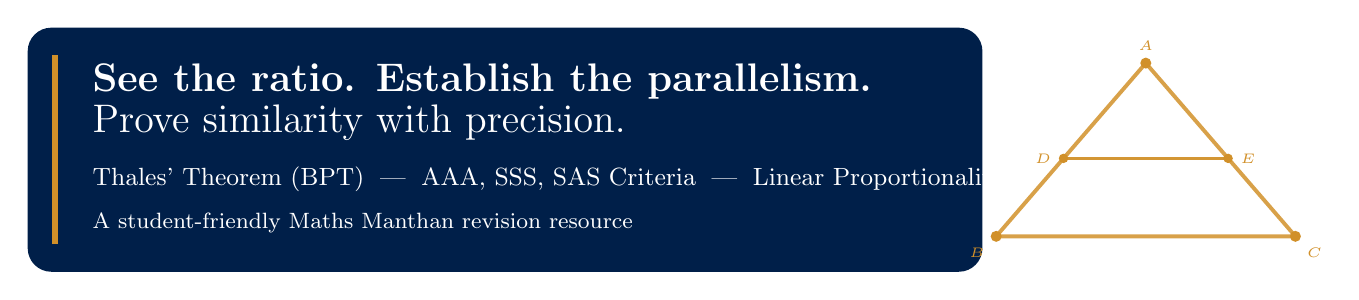
\begin{tikzpicture}
  \fill[navy,rounded corners=3mm] (0,0) rectangle (\textwidth,3.1);
  \draw[gold,line width=2pt] (0.35,0.35)--(0.35,2.75);
  \node[anchor=west,text=white,font=\bfseries\Large] at (0.7,2.42) {See the ratio. Establish the parallelism.};
  \node[anchor=west,text=white,font=\Large] at (0.7,1.90) {Prove similarity with precision.};
  \node[anchor=west,text=white,font=\small] at (0.7,1.18) {Thales' Theorem (BPT) \;|\; AAA, SSS, SAS Criteria \;|\; Linear Proportionalities \;|\; Exam Traps};
  \node[anchor=west,text=white!75,font=\footnotesize] at (0.7,0.62) {A student-friendly Maths Manthan revision resource};
  
  % Geometric Triangle and Parallel Transversal motif in gold
  \coordinate (Top) at (14.2, 2.65);
  \coordinate (LeftB) at (12.3, 0.45);
  \coordinate (RightB) at (16.1, 0.45);
  \draw[gold!85, line width=1.4pt] (Top) -- (LeftB) -- (RightB) -- cycle;
  \coordinate (Dmid) at ($(Top)!0.55!(LeftB)$);
  \coordinate (Emid) at ($(Top)!0.55!(RightB)$);
  \draw[gold!95, line width=1.3pt] (Dmid) -- (Emid);
  \fill[gold] (Top) circle (0.07);
  \fill[gold] (LeftB) circle (0.07);
  \fill[gold] (RightB) circle (0.07);
  \fill[gold] (Dmid) circle (0.06);
  \fill[gold] (Emid) circle (0.06);
  \node[font=\tiny\bfseries\color{gold}, above=1pt] at (Top) {$A$};
  \node[font=\tiny\bfseries\color{gold}, left=1pt] at (Dmid) {$D$};
  \node[font=\tiny\bfseries\color{gold}, right=1pt] at (Emid) {$E$};
  \node[font=\tiny\bfseries\color{gold}, below left=1pt] at (LeftB) {$B$};
  \node[font=\tiny\bfseries\color{gold}, below right=1pt] at (RightB) {$C$};
\end{tikzpicture}

\vspace{3mm}
\begin{minipage}[t]{0.48\textwidth}
  \begin{conceptBox}[title=What this handbook includes,fonttitle=\bfseries\color{navy}]
    \begin{itemize}
      \item Full formal proof of \textbf{Basic Proportionality Theorem (BPT)} and its corollaries.
      \item Rigorous criteria for similarity: \textbf{AAA, AA, SSS, and SAS}.
      \item Linear dimensions: Altitudes, medians, and perimeter invariance ($k$).
      \item Classic board models: Trapezium diagonals, shadows, and right-triangle altitude decomposition.
    \end{itemize}
  \end{conceptBox}
\end{minipage}\hfill
\begin{minipage}[t]{0.48\textwidth}
  \begin{formulaBox}[title=How to use this handbook,fonttitle=\bfseries\color{navy}]
    \raggedright Always state the similarity criterion before writing side ratios. Write triangle vertices in \textbf{strict corresponding order} ($\triangle ABC \sim \triangle DEF$). State the formal justification (e.g. \textit{"By BPT"} or \textit{"By AA similarity"}) at every step to secure full step marks.
  \end{formulaBox}
\end{minipage}

\vspace{1.5mm}
\begin{warningBox}[title=Official CBSE Curriculum Scope (Academic Year 2026--27),fonttitle=\bfseries\color{navy}]
  \textbf{Strict Syllabus Integrity \& Deleted Content:}
  Under the rationalized CBSE 2026--27 curriculum, the \textbf{Area of Similar Triangles Theorem} ($\frac{\text{Area}_1}{\text{Area}_2} = (\frac{s_1}{s_2})^2$) and the \textbf{Formal Proof of Pythagoras Theorem} (and its converse) have been \textbf{permanently excised} from Chapter 6. This handbook covers the complete 100\% prescribed syllabus: BPT, Converse of BPT, and the Similarity Criteria (AAA, SSS, SAS).
  {\scriptsize Source: \href{https://cbseacademic.nic.in/web_material/CurriculumMain27/SecPart1/Maths_SecP1X_2026-27.pdf}{CBSE Secondary Curriculum (2026--27), Unit IV: Geometry}.}
\end{warningBox}

\vfill
\begin{center}
  {\small\bfseries\color{navy}Maths Manthan Tuition Classes}\\
  {\footnotesize\color{muted}contact@mathsmanthan.co.in \quad\textbar\quad +91-8171546558}\\
  {\footnotesize\url{https://mathsmanthan.co.in}}\\[2mm]
  {\scriptsize\color{muted}Prepared for learning and revision \;--\; not an official CBSE publication.}
\end{center}

\clearpage

% =============================================================================
% PAGE 2: MODULE 1 — GEOMETRIC FOUNDATIONS: CONGRUENCE VS. SIMILARITY
% =============================================================================
\thispagestyle{fancy}
\vspace*{0mm}

\chapterbanner{06}{GEOMETRIC FOUNDATIONS: SIMILARITY}{Congruence vs. Similarity, The Scale Factor \& Vertex Correspondence Notation}{\SupportTag}

\subhead{Module 1.1 $\vert$ The Conceptual Leap: Congruence vs. Similarity}

Two geometric figures are:
\begin{itemize}
  \item \textbf{Congruent ($\cong$):} If they have the \textbf{same shape} and the \textbf{same size}. Superimposing one on the other results in a perfect match. (Scale factor $k = 1$).
  \item \textbf{Similar ($\sim$):} If they have the \textbf{same shape}, but not necessarily the same size. One is an exact enlargement or reduction of the other. (Scale factor $k > 0$).
  \item \textbf{Core Axiom:} \textit{All congruent figures are similar, but similar figures need not be congruent.}
\end{itemize}

\subhead{Module 1.2 $\vert$ General Conditions for Similarity of Polygons}

Two polygons with the same number of sides are \textbf{similar} if and only if:
\begin{enumerate}[label=(\roman*)]
  \item All corresponding angles are \textbf{equal} (Equiangular).
  \item All corresponding sides are in the \textbf{same ratio} (Proportional).
\end{enumerate}

\begin{center}
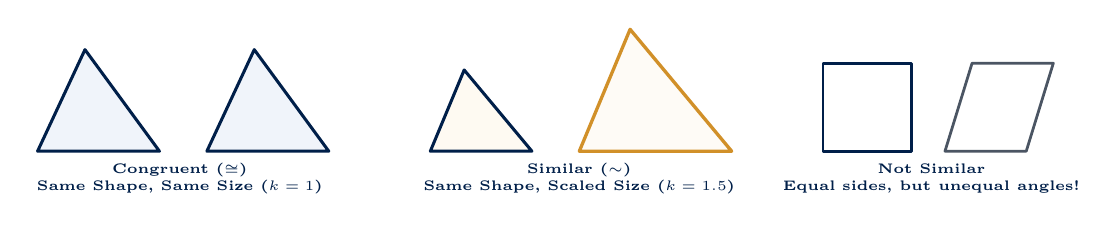
\begin{tikzpicture}[scale=0.86, line cap=round, line join=round]
  % Congruent Triangles (k = 1)
  \begin{scope}[shift={(0,0)}]
    \draw[navy, fill=bluepale, line width=1.1pt] (0,0) -- (1.8,0) -- (0.7,1.5) -- cycle;
    \draw[navy, fill=bluepale, line width=1.1pt] (2.5,0) -- (4.3,0) -- (3.2,1.5) -- cycle;
    \node[font=\tiny\bfseries\color{navy}, align=center] at (2.1,-0.4) {\textbf{Congruent} ($\cong$)\\Same Shape, Same Size ($k=1$)};
  \end{scope}

  % Similar Triangles (k = 1.5)
  \begin{scope}[shift={(5.8,0)}]
    \draw[navy, fill=accentlight, line width=1.1pt] (0,0) -- (1.5,0) -- (0.5,1.2) -- cycle;
    \draw[accent, fill=accentlight!70, line width=1.2pt] (2.2,0) -- (4.45,0) -- (2.95,1.8) -- cycle;
    \node[font=\tiny\bfseries\color{navy}, align=center] at (2.2,-0.4) {\textbf{Similar} ($\sim$)\\Same Shape, Scaled Size ($k = 1.5$)};
  \end{scope}

  % Non-Similar Counter-example (Square vs Rhombus)
  \begin{scope}[shift={(11.6,0)}]
    \draw[navy, line width=1pt] (0,0) rectangle (1.3,1.3);
    \draw[secondary, line width=1pt] (1.8,0) -- (3.0,0) -- (3.4,1.3) -- (2.2,1.3) -- cycle;
    \node[font=\tiny\bfseries\color{reddeep}, align=center] at (1.6,-0.4) {\textbf{Not Similar}\\Equal sides, but unequal angles!};
  \end{scope}
\end{tikzpicture}
\end{center}

\vspace{-1mm}
\subhead{Module 1.3 $\vert$ The Golden Rule of Similarity Notation: Vertex Ordering}

In board examinations, writing the vertices in correct correspondence order is mandatory:

\begin{formulaBox}
  If $\mathbf{\triangle ABC \sim \triangle DEF}$, it means:
  \[
    \boxed{\angle A = \angle D, \quad \angle B = \angle E, \quad \angle C = \angle F}
    \qquad \text{and} \qquad
    \boxed{\frac{AB}{DE} = \frac{BC}{EF} = \frac{CA}{FD} = k}
  \]
  where $k$ is the \textbf{scale factor} (or similarity ratio).
\end{formulaBox}

\begin{warningBox}[title=Critical Board Presentation Trap: Misaligned Letters,fonttitle=\bfseries\color{reddeep}]
  Never write $\triangle ABC \sim \triangle DFE$ if $\angle B = \angle E$ and $\angle C = \angle F$. Swapping vertex letters changes the implied corresponding sides and results in automatic deduction of marks in CBSE step-evaluation.
\end{warningBox}

\clearpage

% =============================================================================
% PAGE 3: MODULE 2 — BASIC PROPORTIONALITY THEOREM (THALES' THEOREM / BPT)
% =============================================================================
\thispagestyle{fancy}
\vspace*{0mm}

\chapterbanner{06}{BASIC PROPORTIONALITY THEOREM (BPT)}{Thales' Theorem: Formal Statement, Construction \& Step-by-Step Board Proof}{\CoreTag}

\subhead{Module 2.1 $\vert$ Official CBSE Theorem Statement}

\begin{formulaBox}
  \textbf{CBSE Theorem 6.1 (Basic Proportionality Theorem / Thales' Theorem):} \\
  \textit{If a line is drawn parallel to one side of a triangle to intersect the other two sides in distinct points, the other two sides are divided in the same ratio.} \quad $\boxed{\text{In } \triangle ABC, \; DE \parallel BC \implies \frac{AD}{DB} = \frac{AE}{EC}}$
\end{formulaBox}

\subhead{Module 2.2 $\vert$ Standard CBSE Board Proof (The Area Ratio Method)}

\begin{minipage}[t]{0.56\textwidth}
  \textbf{Given:} $\triangle ABC$ with line $DE \parallel BC$ intersecting $AB$ at $D$, $AC$ at $E$.\\
  \textbf{To Prove:} $\frac{AD}{DB} = \frac{AE}{EC}$.\\
  \textbf{Construction:} Join $BE$ and $CD$. Draw $EN \perp AB$ and $DM \perp AC$.

  \vspace{0.8mm}
  \textbf{Proof Steps:}
  \begin{enumerate}[leftmargin=4mm, itemsep=1pt]
    \item $\text{Area}(\triangle ADE) = \frac{1}{2} \cdot AD \cdot EN$, \quad $\text{Area}(\triangle BDE) = \frac{1}{2} \cdot DB \cdot EN$. \\
      \textit{($EN$ is the altitude to base $AB$ for both triangles)}.
    \item Ratio:
      $\frac{\text{Area}(\triangle ADE)}{\text{Area}(\triangle BDE)} = \frac{\frac{1}{2} \cdot AD \cdot EN}{\frac{1}{2} \cdot DB \cdot EN} = \frac{AD}{DB} \quad \text{--- (1)}$
    \item Similarly on base $AC$:
      $\frac{\text{Area}(\triangle ADE)}{\text{Area}(\triangle CDE)} = \frac{\frac{1}{2} \cdot AE \cdot DM}{\frac{1}{2} \cdot EC \cdot DM} = \frac{AE}{EC} \quad \text{--- (2)}$
    \item $\triangle BDE$ and $\triangle CDE$ lie on the \textbf{same base} $DE$ and between the \textbf{same parallels} $DE \parallel BC$:
      \[
        \text{Area}(\triangle BDE) = \text{Area}(\triangle CDE) \quad \text{--- (3)}
      \]
    \item From (1), (2), and (3):
      $\mathbf{\frac{AD}{DB} = \frac{AE}{EC}}$. \quad \textbf{[Hence Proved]}
  \end{enumerate}
\end{minipage}\hfill
\begin{minipage}[t]{0.41\textwidth}
  \begin{center}
  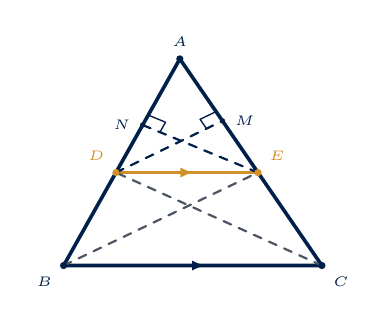
\begin{tikzpicture}[scale=0.82, line cap=round, line join=round]
    \coordinate (A) at (1.8, 3.2);
    \coordinate (B) at (0, 0);
    \coordinate (C) at (4.0, 0);

    \coordinate (D) at ($(A)!0.55!(B)$);
    \coordinate (E) at ($(A)!0.55!(C)$);

    \draw[navy, line width=1.3pt] (A) -- (B) -- (C) -- cycle;
    \draw[accent, line width=1.3pt] (D) -- (E);

    \draw[secondary, line width=0.8pt, dashed] (B) -- (E);
    \draw[secondary, line width=0.8pt, dashed] (C) -- (D);

    \coordinate (N) at ($(A)!0.32!(B)$);
    \coordinate (M) at ($(A)!0.30!(C)$);
    \draw[reddeep, line width=0.8pt, dashed] (E) -- (N);
    \draw[reddeep, line width=0.8pt, dashed] (D) -- (M);

    \draw[reddeep, line width=0.5pt] ($(N)!0.15!(E)$) -- ($(N)!0.15!(E) + (N)!0.15!(A) - (N)$) -- ($(N)!0.15!(A)$);
    \draw[reddeep, line width=0.5pt] ($(M)!0.15!(D)$) -- ($(M)!0.15!(D) + (M)!0.15!(A) - (M)$) -- ($(M)!0.15!(A)$);

    \fill[navy] (A) circle (1.6pt) node[above=1pt, font=\tiny\bfseries\color{navy}]{$A$};
    \fill[navy] (B) circle (1.6pt) node[below left=1pt, font=\tiny\bfseries\color{navy}]{$B$};
    \fill[navy] (C) circle (1.6pt) node[below right=1pt, font=\tiny\bfseries\color{navy}]{$C$};
    \fill[accent] (D) circle (1.6pt) node[above left=1pt, font=\tiny\bfseries\color{accent}]{$D$};
    \fill[accent] (E) circle (1.6pt) node[above right=1pt, font=\tiny\bfseries\color{accent}]{$E$};
    \fill[reddeep] (N) circle (1.2pt) node[left=1pt, font=\tiny\bfseries\color{reddeep}]{$N$};
    \fill[reddeep] (M) circle (1.2pt) node[right=1pt, font=\tiny\bfseries\color{reddeep}]{$M$};

    \draw[-{Latex[scale=0.7]}, accent, line width=0.9pt] ($(D)!0.45!(E)$) -- ($(D)!0.55!(E)$);
    \draw[-{Latex[scale=0.7]}, navy, line width=0.9pt] ($(B)!0.45!(C)$) -- ($(B)!0.55!(C)$);
  \end{tikzpicture}
  \end{center}
\end{minipage}

\vspace{-1mm}
\begin{conceptBox}[title=Pedagogical Keystone: Why Do Oblique Altitudes Work?,fonttitle=\bfseries\color{navy}]
  Notice that $\triangle BDE$ is obtuse-angled. Its altitude from vertex $E$ falls on the line extension of base $BD$ (segment $AB$). Thus $EN$ serves simultaneously as the perpendicular altitude for both acute $\triangle ADE$ and obtuse $\triangle BDE$.
\end{conceptBox}

\clearpage

% =============================================================================
% PAGE 4: MODULE 3 — BPT COROLLARIES & THE CONVERSE OF BPT
% =============================================================================
\thispagestyle{fancy}
\vspace*{0mm}

\chapterbanner{06}{BPT COROLLARIES \& CONVERSE OF THALES}{The Three Algebraic Formulations, Proof by Contradiction \& Mid-Point Specialization}{\CoreTag}

\subhead{Module 3.1 $\vert$ The Three Master Algebraic Forms of BPT}

By applying basic ratio operations (componendo), two additional forms emerge directly:

\begin{center}
\small
\begin{tabularx}{\textwidth}{>{\bfseries\color{navy}}p{28mm} >{\bfseries\color{primary}}c X}
\toprule
\rowcolor{bluepale}Form & Algebraic Identity & Application in Board Exam Problems \\
\midrule
Form 1 (Standard) & $\mathbf{\frac{AD}{DB} = \frac{AE}{EC}}$ & Direct ratio of upper segments to lower segments. Used when all 4 segments are given. \\
Form 2 (Part-to-Whole) & $\mathbf{\frac{AD}{AB} = \frac{AE}{AC}}$ & Add $1$: $\frac{AD}{DB} + 1 = \frac{AE}{EC} + 1 \implies \frac{AB}{DB} = \frac{AC}{EC}$. Inverting gives $\frac{AD}{AB} = \frac{AE}{AC}$. \\
Form 3 (Lower-to-Whole) & $\mathbf{\frac{DB}{AB} = \frac{EC}{AC}}$ & Compares bottom segments directly to the entire side lengths $AB$ and $AC$. \\
\bottomrule
\end{tabularx}
\end{center}

\subhead{Module 3.2 $\vert$ Converse of Basic Proportionality Theorem (Theorem 6.2)}

\begin{minipage}[t]{0.56\textwidth}
  \begin{formulaBox}
    \textbf{CBSE Theorem 6.2 (Converse of BPT):} \\
    \textit{If a line divides two sides of a triangle in the same ratio, then the line is parallel to the third side.}
    \[
      \boxed{\text{In } \triangle ABC, \quad \frac{AD}{DB} = \frac{AE}{EC} \implies DE \parallel BC}
    \]
  \end{formulaBox}
  \textbf{Proof by Contradiction Summary:}
  \begin{enumerate}[leftmargin=4.5mm, itemsep=1.2pt]
    \item Suppose line $DE$ is \textbf{not} parallel to $BC$.
    \item Draw line $DE' \parallel BC$ meeting $AC$ at $E'$.
    \item By BPT: $\frac{AD}{DB} = \frac{AE'}{E'C}$. But given: $\frac{AD}{DB} = \frac{AE}{EC}$.
    \item Hence: $\frac{AE}{EC} = \frac{AE'}{E'C} \implies \frac{AE+EC}{EC} = \frac{AE'+E'C}{E'C} \implies \frac{AC}{EC} = \frac{AC}{E'C}$.
    \item Thus $EC = E'C$, which means \textbf{$E$ and $E'$ coincide}.
    \item Therefore, $DE \parallel BC$. \quad \textbf{[Q.E.D.]}
  \end{enumerate}
\end{minipage}\hfill
\begin{minipage}[t]{0.41\textwidth}
  \begin{center}
  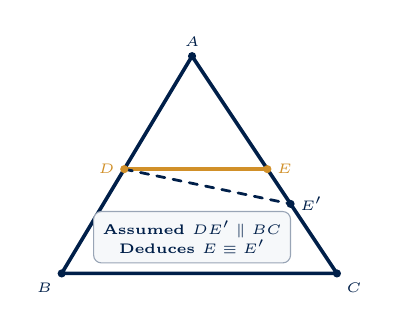
\begin{tikzpicture}[scale=0.92, line cap=round, line join=round]
    \coordinate (A) at (1.8, 3.0);
    \coordinate (B) at (0, 0);
    \coordinate (C) at (3.8, 0);

    \coordinate (D) at ($(A)!0.52!(B)$);
    \coordinate (E) at ($(A)!0.52!(C)$);
    \coordinate (Eprime) at ($(A)!0.68!(C)$);

    \draw[navy, line width=1.3pt] (A) -- (B) -- (C) -- cycle;
    \draw[accent, line width=1.3pt] (D) -- (E);
    \draw[reddeep, line width=1pt, dashed] (D) -- (Eprime);

    \fill[navy] (A) circle (1.6pt) node[above, font=\tiny\bfseries]{$A$};
    \fill[navy] (B) circle (1.6pt) node[below left, font=\tiny\bfseries]{$B$};
    \fill[navy] (C) circle (1.6pt) node[below right, font=\tiny\bfseries]{$C$};
    \fill[accent] (D) circle (1.6pt) node[left, font=\tiny\bfseries]{$D$};
    \fill[accent] (E) circle (1.6pt) node[right, font=\tiny\bfseries\color{accent}]{$E$};
    \fill[reddeep] (Eprime) circle (1.6pt) node[right, font=\tiny\bfseries\color{reddeep}]{$E'$};

    \node[draw=reddeep!40, fill=redpale, rounded corners=1mm, font=\tiny\bfseries\color{navy}, align=center] at (1.8, 0.5) {
      Assumed $DE' \parallel BC$\\
      Deduces $E \equiv E'$
    };
  \end{tikzpicture}
  \end{center}
\end{minipage}

\vspace{-1mm}
\subhead{Module 3.3 $\vert$ Mid-Point Theorem as a Direct Specialization of BPT}

\begin{successBox}[title=Connecting Class 9 and Class 10 Geometry,fonttitle=\bfseries\color{green}]
  If $D$ and $E$ are mid-points of $AB$ and $AC$, then $AD = DB$ and $AE = EC$, so $\frac{AD}{DB} = \frac{AE}{EC} = 1$.
  By the \textbf{Converse of BPT}, $DE \parallel BC$. Thus, the Class 9 Mid-Point Theorem is simply BPT at $k = 1$.
\end{successBox}

\clearpage

% =============================================================================
% PAGE 5: MODULE 4 — BPT PROBLEM-SOLVING PROTOCOLS & TRAPEZIUM MODELS
% =============================================================================
\thispagestyle{fancy}
\vspace*{0mm}

\chapterbanner{06}{BPT PROBLEM-SOLVING \& TRAPEZIUM MODELS}{Algebraic Protocols for Unknown $x$ \& The Diagonal Proportionality Theorem}{\WorkedTag}

\subhead{Module 4.1 $\vert$ The Algebraic Protocol for Solving BPT Problems}

\begin{itemize}[itemsep=1pt]
  \item \textbf{Step 1:} Verify that $DE \parallel BC$ is stated. \quad \textbf{Step 2:} Write $\frac{AD}{DB} = \frac{AE}{EC}$ citing \textit{"(By BPT)"}.
  \item \textbf{Step 3:} Substitute algebraic expressions, cross-multiply, and solve the equation.
  \item \textbf{Step 4:} Reject extraneous negative roots (segment lengths must remain strictly positive).
\end{itemize}

\subhead{Module 4.2 $\vert$ Worked Archetype 1: Solving Quadratic BPT Equations}

\begin{conceptBox}[title=Worked Archetype 1: Determining Variable $x$ Using BPT,fonttitle=\bfseries\color{navy}]
  \textbf{Problem:} In $\triangle ABC$, $DE \parallel BC$. If $AD = x$, $DB = x - 2$, $AE = x + 2$, and $EC = x - 1$, find $x$.\\
  \textbf{Solution:}
  By \textbf{Basic Proportionality Theorem}: $\frac{AD}{DB} = \frac{AE}{EC} \implies \frac{x}{x - 2} = \frac{x + 2}{x - 1}$.\\
  Cross-multiplying: $x(x - 1) = (x - 2)(x + 2) \implies x^2 - x = x^2 - 4 \implies -x = -4 \implies \mathbf{x = 4\text{ cm}}$.
\end{conceptBox}

\subhead{Module 4.3 $\vert$ The Classic Trapezium Proportionality Theorem}

\begin{minipage}[t]{0.56\textwidth}
  \textbf{CBSE Standard 3-Mark Theorem:} \\
  \textit{The diagonals of a trapezium divide each other proportionally.}
  \[
    \boxed{\text{In trapezium } ABCD \text{ with } AB \parallel CD, \quad \mathbf{\frac{AO}{OC} = \frac{BO}{OD}}}
  \]
  \textbf{Proof Construction:}
  Through point $O$, draw line $OE \parallel AB \parallel CD$ meeting $AD$ at $E$.
  \begin{enumerate}[leftmargin=4mm, itemsep=1pt]
    \item In $\triangle ADC$, since $OE \parallel CD$:
      $\frac{AE}{ED} = \frac{AO}{OC} \quad \text{--- (1) [By BPT]}$
    \item In $\triangle DAB$, since $EO \parallel AB$:
      $\frac{ED}{AE} = \frac{OD}{BO} \implies \frac{AE}{ED} = \frac{BO}{OD} \quad \text{--- (2)}$
    \item Equating (1) and (2): $\mathbf{\frac{AO}{OC} = \frac{BO}{OD}}$. \textbf{[Q.E.D.]}
  \end{enumerate}
  \textit{Converse:} If $\frac{AO}{OC} = \frac{BO}{OD}$, then $ABCD$ is a \textbf{trapezium} ($AB \parallel CD$).
\end{minipage}\hfill
\begin{minipage}[t]{0.41\textwidth}
  \begin{center}
  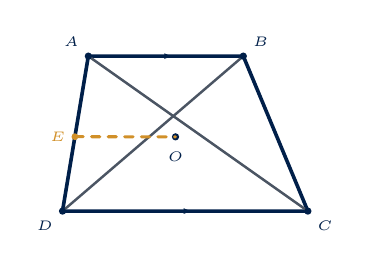
\begin{tikzpicture}[scale=0.82, line cap=round, line join=round]
    \coordinate (A) at (0.4, 2.4);
    \coordinate (B) at (2.8, 2.4);
    \coordinate (C) at (3.8, 0);
    \coordinate (D) at (0, 0);

    \draw[navy, line width=1.3pt] (A) -- (B) -- (C) -- (D) -- cycle;
    \draw[secondary, line width=0.9pt] (A) -- (C);
    \draw[secondary, line width=0.9pt] (B) -- (D);

    \coordinate (O) at (1.75, 1.15);
    \fill[primary] (O) circle (1.6pt) node[below=2pt, font=\tiny\bfseries\color{primary}]{$O$};

    \coordinate (E) at ($(A)!0.52!(D)$);
    \draw[accent, line width=1.1pt, dashed] (E) -- (O);
    \fill[accent] (E) circle (1.5pt) node[left, font=\tiny\bfseries\color{accent}]{$E$};

    \fill[navy] (A) circle (1.6pt) node[above left, font=\tiny\bfseries]{$A$};
    \fill[navy] (B) circle (1.6pt) node[above right, font=\tiny\bfseries]{$B$};
    \fill[navy] (C) circle (1.6pt) node[below right, font=\tiny\bfseries]{$C$};
    \fill[navy] (D) circle (1.6pt) node[below left, font=\tiny\bfseries]{$D$};

    \draw[-{Latex[scale=0.6]}, navy] (1.5,2.4) -- (1.7,2.4);
    \draw[-{Latex[scale=0.6]}, navy] (1.8,0) -- (2.0,0);
  \end{tikzpicture}
  \end{center}
\end{minipage}

\clearpage

% =============================================================================
% PAGE 6: MODULE 5 — TRIANGLE SIMILARITY CRITERIA: AAA AND AA
% =============================================================================
\thispagestyle{fancy}
\vspace*{0mm}

\chapterbanner{06}{SIMILARITY CRITERIA: AAA \& AA}{Equiangularity Mechanics, The 2-Angle Board Shortcut \& Shadow Models}{\CoreTag}

\subhead{Module 5.1 $\vert$ The AAA Similarity Criterion (Theorem 6.3)}

\begin{formulaBox}
  \textbf{CBSE Theorem 6.3 (AAA Similarity Criterion):} \\
  \textit{If in two triangles, corresponding angles are equal, then their corresponding sides are in the same ratio, and hence the two triangles are similar.}
  \[
    \boxed{\angle A = \angle D, \quad \angle B = \angle E, \quad \angle C = \angle F \implies \triangle ABC \sim \triangle DEF}
  \]
\end{formulaBox}

\subhead{Module 5.2 $\vert$ The Indispensable AA Similarity Shortcut (Board Exam Standard)}

\begin{minipage}[t]{0.56\textwidth}
  In any triangle, the sum of all three interior angles is $180^\circ$. \\
  If two angles of $\triangle ABC$ equal two angles of $\triangle DEF$:
  \[
    \angle A = \angle D \quad \text{and} \quad \angle B = \angle E
  \]
  Then the third angles are automatically equal:
  \[
    \angle C = 180^\circ - (\angle A + \angle B) = 180^\circ - (\angle D + \angle E) = \angle F
  \]
  \begin{successBox}[title=Golden Exam Rule: Use AA Similarity,fonttitle=\bfseries\color{green}]
    Proving \textbf{any two pairs of corresponding angles equal} is sufficient to declare similarity by the \textbf{AA criterion}.
  \end{successBox}
\end{minipage}\hfill
\begin{minipage}[t]{0.41\textwidth}
  \begin{center}
  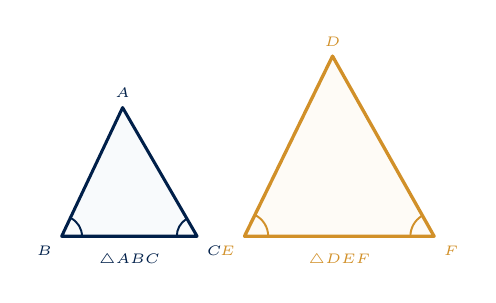
\begin{tikzpicture}[scale=0.86, line cap=round, line join=round]
    % Triangle ABC
    \coordinate (A) at (0.9, 1.9);
    \coordinate (B) at (0, 0);
    \coordinate (C) at (2.0, 0);
    \draw[navy, fill=bluepale!50, line width=1.1pt] (A) -- (B) -- (C) -- cycle;

    % Triangle DEF (scaled 1.4)
    \coordinate (D) at (4.0, 2.66);
    \coordinate (E) at (2.7, 0);
    \coordinate (F) at (5.5, 0);
    \draw[accent, fill=accentlight!70, line width=1.2pt] (D) -- (E) -- (F) -- cycle;

    \draw[navy, line width=0.7pt] (B) ++(0:0.3) arc (0:63:0.3);
    \draw[accent, line width=0.7pt] (E) ++(0:0.35) arc (0:63:0.35);
    \draw[navy, line width=0.7pt] (C) ++(180:0.3) arc (180:122:0.3);
    \draw[accent, line width=0.7pt] (F) ++(180:0.35) arc (180:122:0.35);

    \node[above, font=\tiny\bfseries\color{navy}] at (A) {$A$};
    \node[below left, font=\tiny\bfseries\color{navy}] at (B) {$B$};
    \node[below right, font=\tiny\bfseries\color{navy}] at (C) {$C$};
    \node[above, font=\tiny\bfseries\color{accent}] at (D) {$D$};
    \node[below left, font=\tiny\bfseries\color{accent}] at (E) {$E$};
    \node[below right, font=\tiny\bfseries\color{accent}] at (F) {$F$};

    \node[font=\tiny\bfseries\color{primary}] at (1.0,-0.35) {$\triangle ABC$};
    \node[font=\tiny\bfseries\color{accent}] at (4.1,-0.35) {$\triangle DEF$};
  \end{tikzpicture}
  \end{center}
\end{minipage}

\subhead{Module 5.3 $\vert$ Worked Archetype 2: The Vertical Pole \& Tower Shadow Problem}

\begin{conceptBox}[title=Worked Archetype 2: Tower and Pole Shadow Model,fonttitle=\bfseries\color{navy}]
  \textbf{Problem:} A vertical pole of $6\text{ m}$ casts a shadow of $4\text{ m}$. At the same time, a tower casts a shadow of $28\text{ m}$. Find the tower's height $h$.\\
  \textbf{Solution:}
  $\angle B = \angle Q = 90^\circ$ and $\angle C = \angle R$ (Sun's elevation is identical at same time).
  By \textbf{AA similarity}, $\triangle ABC \sim \triangle PQR \implies \frac{AB}{PQ} = \frac{BC}{QR} \implies \frac{6}{h} = \frac{4}{28} \implies \frac{6}{h} = \frac{1}{7} \implies \mathbf{h = 42\text{ m}}$.
\end{conceptBox}

\clearpage

% =============================================================================
% PAGE 7: MODULE 6 — TRIANGLE SIMILARITY CRITERIA: SSS AND SAS
% =============================================================================
\thispagestyle{fancy}
\vspace*{0mm}

\chapterbanner{06}{SIMILARITY CRITERIA: SSS \& SAS}{Side-Ratio Equiangularity, The Included-Angle Rule \& The SSA Trap Alert}{\CoreTag}

\subhead{Module 6.1 $\vert$ The SSS Similarity Criterion (Theorem 6.4)}

\begin{formulaBox}
  \textbf{CBSE Theorem 6.4 (SSS Similarity Criterion):} \\
  \textit{If in two triangles, sides of one triangle are proportional to the sides of the other triangle, then their corresponding angles are equal and hence the two triangles are similar.}
  \[
    \boxed{\frac{AB}{DE} = \frac{BC}{EF} = \frac{CA}{FD} = k \implies \triangle ABC \sim \triangle DEF}
  \]
\end{formulaBox}

\subhead{Module 6.2 $\vert$ The SAS Similarity Criterion (Theorem 6.5) \& The "Included Angle" Rule}

\begin{formulaBox}
  \textbf{CBSE Theorem 6.5 (SAS Similarity Criterion):} \\
  \textit{If one angle of a triangle equals one angle of another triangle and the sides including these angles are proportional, then the two triangles are similar.}
  \[
    \boxed{\angle A = \angle D \quad \text{and} \quad \frac{AB}{DE} = \frac{AC}{DF} \implies \triangle ABC \sim \triangle DEF}
  \]
\end{formulaBox}

\begin{center}
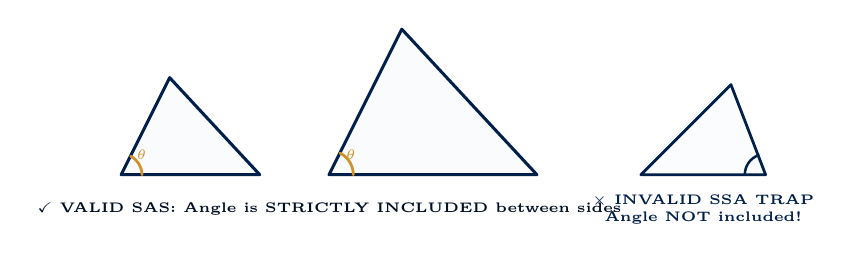
\begin{tikzpicture}[scale=0.88, line cap=round, line join=round]
  % Valid SAS
  \begin{scope}[shift={(0,0)}]
    \draw[navy, fill=bluepale!40, line width=1.1pt] (0,0) -- (2.0,0) -- (0.7,1.4) -- cycle;
    \draw[accent, line width=1pt] (0,0) ++(0:0.3) arc (0:63:0.3);
    \node[above right, font=\tiny\bfseries\color{accent}] at (0.08,0.08) {$\theta$};

    \draw[navy, fill=bluepale!40, line width=1.1pt] (3.0,0) -- (6.0,0) -- (4.05,2.1) -- cycle;
    \draw[accent, line width=1pt] (3.0,0) ++(0:0.35) arc (0:63:0.35);
    \node[above right, font=\tiny\bfseries\color{accent}] at (3.1,0.08) {$\theta$};

    \node[font=\tiny\bfseries\color{green!50!black}, align=center] at (3.0,-0.5) {$\checkmark$ \textbf{VALID SAS: Angle is STRICTLY INCLUDED between sides}};
  \end{scope}

  % Invalid SSA Trap
  \begin{scope}[shift={(7.5,0)}]
    \draw[reddeep, fill=redpale!40, line width=1pt] (0,0) -- (1.8,0) -- (1.3,1.3) -- cycle;
    \draw[reddeep, line width=0.9pt] (1.8,0) ++(180:0.3) arc (180:110:0.3);
    \node[font=\tiny\bfseries\color{reddeep}, align=center] at (0.9,-0.5) {$\times$ \textbf{INVALID SSA TRAP}\\Angle NOT included!};
  \end{scope}
\end{tikzpicture}
\end{center}

\vspace{-1mm}
\subhead{Module 6.3 $\vert$ Worked Archetype 3: The Intersecting Chords / Butterfly Configuration}

\begin{conceptBox}[title=Worked Archetype 3: Intersecting Diagonals Model,fonttitle=\bfseries\color{navy}]
  \textbf{Problem:} Line segments $AB$ and $CD$ intersect at $O$ with $OA = 4\text{ cm}, OB = 6\text{ cm}, OC = 8\text{ cm}$, and $OD = 12\text{ cm}$. Prove $\triangle AOC \sim \triangle BOD$.\\
  \textbf{Solution:}
  Compare side ratios: $\frac{OA}{OB} = \frac{4}{6} = \frac{2}{3}$ and $\frac{OC}{OD} = \frac{8}{12} = \frac{2}{3} \implies \frac{OA}{OB} = \frac{OC}{OD}$.\\
  Included angles: $\angle AOC = \angle BOD$ (vertically opposite). By \textbf{SAS similarity}: $\mathbf{\triangle AOC \sim \triangle BOD}$.
\end{conceptBox}

\clearpage

% =============================================================================
% PAGE 8: MODULE 7 — LINEAR PROPORTIONALITIES IN SIMILAR TRIANGLES
% =============================================================================
\thispagestyle{fancy}
\vspace*{0mm}

\chapterbanner{06}{LINEAR PROPORTIONALITIES IN SIMILAR TRIANGLES}{Altitudes, Medians, Perimeters \& The Master Linear Invariance Ratio}{\WorkedTag}

\subhead{Module 8.1 $\vert$ The Master Linear Invariance Theorem}

When two triangles are similar, the scale factor $k$ governs \textbf{every linear measure} of the triangles:

\begin{formulaBox}
  If $\mathbf{\triangle ABC \sim \triangle DEF}$ with scale factor $k = \frac{AB}{DE} = \frac{BC}{EF} = \frac{CA}{FD}$:
  \[
    \boxed{\frac{\text{Perimeter}(\triangle ABC)}{\text{Perimeter}(\triangle DEF)} = \frac{\text{Altitude } h_1}{\text{Altitude } h_2} = \frac{\text{Median } m_1}{\text{Median } m_2} = \frac{\text{Inradius } r_1}{\text{Inradius } r_2} = \mathbf{k}}
  \]
\end{formulaBox}

\subhead{Module 8.2 $\vert$ Standard CBSE Board Proofs (High-Yield 3-Markers)}

\begin{minipage}[t]{0.54\textwidth}
  \textbf{Theorem A: Ratio of Altitudes = Ratio of Sides}\\
  Let $AM \perp BC$ and $DN \perp EF$.
  \begin{enumerate}[leftmargin=4.5mm, itemsep=1.2pt]
    \item In $\triangle ABM$ and $\triangle DEN$:
      $\angle B = \angle E$ and $\angle AMB = \angle DNE = 90^\circ$.
    \item By \textbf{AA similarity}: $\triangle ABM \sim \triangle DEN$.
    \item Hence: $\mathbf{\frac{AM}{DN} = \frac{AB}{DE} = k}$. \textbf{[Q.E.D.]}
  \end{enumerate}

  \vspace{0.8mm}
  \textbf{Theorem B: Ratio of Medians = Ratio of Sides}\\
  Let $AP$ and $DQ$ be medians to $BC$ and $EF$.
  \begin{enumerate}[leftmargin=4.5mm, itemsep=1.2pt]
    \item Since $P, Q$ are mid-points:
      $\frac{BP}{EQ} = \frac{\frac{1}{2}BC}{\frac{1}{2}EF} = \frac{BC}{EF} = \frac{AB}{DE}$.
    \item Also $\angle B = \angle E$.
    \item By \textbf{SAS similarity}: $\triangle ABP \sim \triangle DEQ$.
    \item Hence: $\mathbf{\frac{AP}{DQ} = \frac{AB}{DE} = k}$. \textbf{[Q.E.D.]}
  \end{enumerate}
\end{minipage}\hfill
\begin{minipage}[t]{0.43\textwidth}
  \begin{center}
  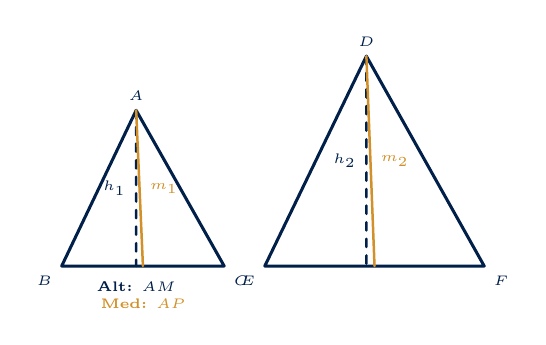
\begin{tikzpicture}[scale=0.86, line cap=round, line join=round]
    % Triangle ABC
    \coordinate (A) at (1.1, 2.3);
    \coordinate (B) at (0, 0);
    \coordinate (C) at (2.4, 0);
    \draw[navy, line width=1.1pt] (A) -- (B) -- (C) -- cycle;
    \draw[reddeep, line width=0.9pt, dashed] (A) -- (1.1, 0) node[midway, left, font=\tiny\bfseries]{$h_1$};
    \draw[accent, line width=0.9pt] (A) -- (1.2, 0) node[midway, right, font=\tiny\bfseries]{$m_1$};

    % Triangle DEF (scaled 1.35)
    \coordinate (D) at (4.5, 3.1);
    \coordinate (E) at (3.0, 0);
    \coordinate (F) at (6.24, 0);
    \draw[navy, line width=1.1pt] (D) -- (E) -- (F) -- cycle;
    \draw[reddeep, line width=0.9pt, dashed] (D) -- (4.5, 0) node[midway, left, font=\tiny\bfseries]{$h_2$};
    \draw[accent, line width=0.9pt] (D) -- (4.62, 0) node[midway, right, font=\tiny\bfseries]{$m_2$};

    \node[above, font=\tiny\bfseries\color{navy}] at (A) {$A$};
    \node[below left, font=\tiny\bfseries\color{navy}] at (B) {$B$};
    \node[below right, font=\tiny\bfseries\color{navy}] at (C) {$C$};
    \node[above, font=\tiny\bfseries\color{navy}] at (D) {$D$};
    \node[below left, font=\tiny\bfseries\color{navy}] at (E) {$E$};
    \node[below right, font=\tiny\bfseries\color{navy}] at (F) {$F$};

    \node[font=\tiny\bfseries\color{reddeep}] at (1.1,-0.3) {Alt: $AM$};
    \node[font=\tiny\bfseries\color{accent}] at (1.2,-0.55) {Med: $AP$};
  \end{tikzpicture}
  \end{center}
\end{minipage}

\vspace{-1mm}
\subhead{Module 8.3 $\vert$ Ratio of Perimeters Proof}

By Componendo / Ratio Addition: If $\frac{a_1}{a_2} = \frac{b_1}{b_2} = \frac{c_1}{c_2} = k$, then:
\[
  \frac{\text{Perimeter}_1}{\text{Perimeter}_2} = \frac{a_1 + b_1 + c_1}{a_2 + b_2 + c_2} = \frac{k a_2 + k b_2 + k c_2}{a_2 + b_2 + c_2} = \frac{k(a_2 + b_2 + c_2)}{a_2 + b_2 + c_2} = \mathbf{k}.
\]

\clearpage

% =============================================================================
% PAGE 9: MODULE 8 — WORKED BOARD-EXAM MASTER MODELS
% =============================================================================
\thispagestyle{fancy}
\vspace*{0mm}

\chapterbanner{06}{WORKED BOARD-EXAM MASTER MODELS}{Right-Triangle Altitude Decomposition \& The Walking Person Shadow Model}{\WorkedTag}

\subhead{Module 9.1 $\vert$ Master Model 1: Right-Triangle Altitude Decomposition}

\begin{minipage}[t]{0.56\textwidth}
  \textbf{The Geometric Mean Theorem:} \\
  In $\triangle ABC$ right-angled at $B$, with altitude $BD \perp AC$:
  \begin{enumerate}[leftmargin=4.5mm, itemsep=1.5pt]
    \item $\triangle ADB \sim \triangle ABC$ \quad \textit{(By AA: $\angle A$ common, $\angle ADB = 90^\circ$)}.
    \item $\triangle BDC \sim \triangle ABC$ \quad \textit{(By AA: $\angle C$ common, $\angle BDC = 90^\circ$)}.
    \item $\mathbf{\triangle ADB \sim \triangle BDC}$ \quad \textit{(Both similar to $\triangle ABC$)}.
  \end{enumerate}

  \textbf{Four Master Metric Relations:}
  \[
    \boxed{\mathbf{BD^2 = AD \cdot DC}} \quad \text{(Altitude Theorem)}
  \]
  \[
    \boxed{\mathbf{AB^2 = AD \cdot AC}} \qquad \boxed{\mathbf{BC^2 = CD \cdot AC}}
  \]
  \[
    \boxed{\mathbf{AB \cdot BC = AC \cdot BD}} \quad \text{(Area Identity)}
  \]
\end{minipage}\hfill
\begin{minipage}[t]{0.41\textwidth}
  \begin{center}
  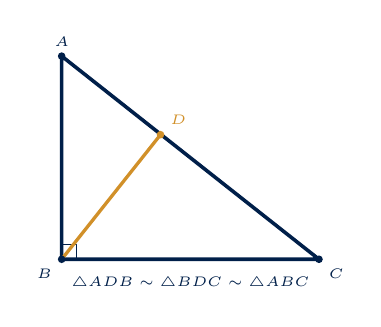
\begin{tikzpicture}[scale=0.86, line cap=round, line join=round]
    \coordinate (B) at (0,0);
    \coordinate (A) at (0,3.0);
    \coordinate (C) at (3.8,0);

    \draw[navy, line width=1.3pt] (A) -- (B) -- (C) -- cycle;
    \draw[navy, line width=0.6pt] (0.22,0) -- (0.22,0.22) -- (0,0.22);

    \coordinate (D) at (1.46, 1.84);
    \draw[accent, line width=1.2pt] (B) -- (D);

    \fill[navy] (A) circle (1.6pt) node[above, font=\tiny\bfseries]{$A$};
    \fill[navy] (B) circle (1.6pt) node[below left, font=\tiny\bfseries]{$B$};
    \fill[navy] (C) circle (1.6pt) node[below right, font=\tiny\bfseries]{$C$};
    \fill[accent] (D) circle (1.6pt) node[above right, font=\tiny\bfseries\color{accent}]{$D$};

    \node[font=\tiny\bfseries\color{primary}] at (1.9,-0.35) {$\triangle ADB \sim \triangle BDC \sim \triangle ABC$};
  \end{tikzpicture}
  \end{center}
\end{minipage}

\subhead{Module 9.2 $\vert$ Master Model 2: The Walking Person Shadow Model (CBSE Standard 4-Marker)}

\begin{conceptBox}[title=Worked Archetype 4: Moving Person Shadow Protocol,fonttitle=\bfseries\color{navy}]
  \textbf{Problem:} A girl of height $90\text{ cm}$ ($0.9\text{ m}$) walks away from a $3.6\text{ m}$ lamppost at $1.2\text{ m/s}$. Find shadow length after 4 seconds.\\
  \textbf{Solution:}
  \begin{enumerate}[leftmargin=4.5mm, itemsep=1.2pt]
    \item Distance walked $BD = 1.2\text{ m/s} \times 4\text{ s} = 4.8\text{ m}$. Let shadow $DE = s$.
    \item In $\triangle ABE$ and $\triangle CDE$: $\angle B = \angle D = 90^\circ$ and $\angle E$ is common.
    \item By \textbf{AA similarity}: $\triangle ABE \sim \triangle CDE \implies \frac{AB}{CD} = \frac{BE}{DE} \implies \frac{3.6}{0.9} = \frac{4.8 + s}{s}$.
    \item $4 = \frac{4.8 + s}{s} \implies 4s = 4.8 + s \implies 3s = 4.8 \implies \mathbf{s = 1.6\text{ m}}$ ($160\text{ cm}$).
  \end{enumerate}
\end{conceptBox}

\clearpage

% =============================================================================
% PAGE 10: MODULE 9 — ENRICHMENT & GEOMETRIC BRIDGES
% =============================================================================
\thispagestyle{fancy}
\vspace*{0mm}

\chapterbanner{06}{ENRICHMENT \& GEOMETRIC BRIDGES}{Pythagoras via Similarity, Internal Angle Bisector \& Competitive Edges}{\ExtensionTag}

\subhead{Module 10.1 $\vert$ The 3-Line Similarity Derivation of Pythagoras Theorem}

Although the axiomatic textbook proof is deleted from CBSE 2026--27, understanding its similarity derivation bridges geometry with algebra:

\begin{minipage}[t]{0.56\textwidth}
  \textbf{The 3-Line Derivation:}
  \begin{enumerate}[leftmargin=4mm, itemsep=1.2pt]
    \item In right $\triangle ABC$ ($\angle B = 90^\circ$) with altitude $BD \perp AC$:
    \item $\triangle ADB \sim \triangle ABC \implies \frac{AB}{AC} = \frac{AD}{AB} \implies \mathbf{AB^2 = AD \cdot AC}$ --- (1)
    \item $\triangle BDC \sim \triangle ABC \implies \frac{BC}{AC} = \frac{CD}{BC} \implies \mathbf{BC^2 = CD \cdot AC}$ --- (2)
    \item Adding (1) + (2):
      $AB^2 + BC^2 = AC(AD + CD) = AC \cdot AC = \mathbf{AC^2}$.
  \end{enumerate}
\end{minipage}\hfill
\begin{minipage}[t]{0.41\textwidth}
  \begin{center}
  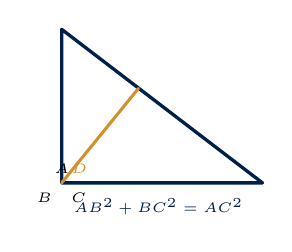
\begin{tikzpicture}[scale=0.75, line cap=round, line join=round]
    \coordinate (B) at (0,0);
    \coordinate (A) at (0,2.6);
    \coordinate (C) at (3.4,0);

    \draw[navy, line width=1.2pt] (A) -- (B) -- (C) -- cycle;
    \coordinate (D) at (1.3, 1.6);
    \draw[accent, line width=1.1pt] (B) -- (D);

    \node[above, font=\tiny\bfseries]{$A$};
    \node[below left, font=\tiny\bfseries]{$B$};
    \node[below right, font=\tiny\bfseries]{$C$};
    \node[above right, font=\tiny\bfseries\color{accent}]{$D$};

    \node[font=\tiny\bfseries\color{navy}, align=center] at (1.7,-0.4) {
      $AB^2 + BC^2 = AC^2$
    };
  \end{tikzpicture}
  \end{center}
\end{minipage}

\vspace{-1mm}
\subhead{Module 10.2 $\vert$ The Internal Angle Bisector Theorem (Competitive Bridge)}

\begin{minipage}[t]{0.56\textwidth}
  \begin{formulaBox}
    \textbf{Internal Angle Bisector Theorem:} \\
    \textit{The internal bisector of an angle of a triangle divides the opposite side in the ratio of the containing sides.}
    \[
      \boxed{\text{In } \triangle ABC, \; AD \text{ bisects } \angle A \implies \mathbf{\frac{BD}{DC} = \frac{AB}{AC}}}
    \]
  \end{formulaBox}
  \textbf{Proof via BPT:} Draw $CE \parallel DA$ meeting $BA$ produced at $E$. $\angle AEC = \angle BAD$ (corr.) and $\angle ACE = \angle CAD$ (alt.). Thus $AE = AC$. By BPT on $\triangle BCE$: $\frac{BD}{DC} = \frac{BA}{AE} = \frac{AB}{AC}$.
\end{minipage}\hfill
\begin{minipage}[t]{0.41\textwidth}
  \begin{center}
  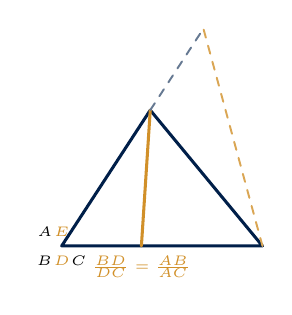
\begin{tikzpicture}[scale=0.75, line cap=round, line join=round]
    \coordinate (A) at (1.5, 2.3);
    \coordinate (B) at (0, 0);
    \coordinate (C) at (3.4, 0);

    \draw[navy, line width=1.1pt] (A) -- (B) -- (C) -- cycle;
    \coordinate (D) at (1.35, 0);
    \draw[accent, line width=1.1pt] (A) -- (D);

    \coordinate (E) at (2.4, 3.68);
    \draw[navy!60, line width=0.7pt, dashed] (A) -- (E);
    \draw[accent!80, line width=0.7pt, dashed] (C) -- (E);

    \node[above left, font=\tiny\bfseries]{$A$};
    \node[below left, font=\tiny\bfseries]{$B$};
    \node[below right, font=\tiny\bfseries]{$C$};
    \node[below, font=\tiny\bfseries\color{accent}]{$D$};
    \node[above, font=\tiny\bfseries\color{accent}]{$E$};

    \node[font=\tiny\bfseries\color{accent}] at (1.35,-0.35) {$\frac{BD}{DC} = \frac{AB}{AC}$};
  \end{tikzpicture}
  \end{center}
\end{minipage}

\clearpage

% =============================================================================
% PAGE 11: MODULE 10 — MASTER SUMMARY & SIMILARITY DECISION MATRIX
% =============================================================================
\thispagestyle{fancy}
\vspace*{0mm}

\chapterbanner{06}{MASTER SUMMARY \& DECISION ALGORITHM}{Comprehensive Similarity Comparison Matrix \& 10-Second Problem Solver}{\ReferenceTag}

\subhead{Module 11.1 $\vert$ Comprehensive Theorem \& Criteria Repository}

\begin{center}
\small
\begin{tabularx}{\textwidth}{>{\bfseries\color{navy}}p{28mm} >{\bfseries\color{primary}}p{42mm} X}
\toprule
\rowcolor{bluepale}Theorem / Criterion & Core Mathematical Condition & Key Exam Application \\
\midrule
BPT (Thales') & $DE \parallel BC \implies \frac{AD}{DB} = \frac{AE}{EC}$ & Finding unknown side segments when parallel transversal is given. \\
Converse of BPT & $\frac{AD}{DB} = \frac{AE}{EC} \implies DE \parallel BC$ & Proving a line segment is parallel to a triangle base. \\
AA Criterion & $\angle A = \angle D, \; \angle B = \angle E$ & The most frequent board shortcut (e.g., shadows, vertical lines). \\
SSS Criterion & $\frac{AB}{DE} = \frac{BC}{EF} = \frac{CA}{FD}$ & Proving triangles similar when all 3 side lengths/ratios are given. \\
SAS Criterion & $\angle A = \angle D, \; \frac{AB}{DE} = \frac{AC}{DF}$ & Used when 2 pairs of sides and their strictly \textbf{included} angle match. \\
Trapezium Theorem & $\frac{AO}{OC} = \frac{BO}{OD}$ & Calculating intersection segments in trapezium diagonals. \\
Linear Invariance & $\frac{P_1}{P_2} = \frac{h_1}{h_2} = \frac{m_1}{m_2} = \frac{\text{side}_1}{\text{side}_2}$ & Rapid calculation of perimeter, altitude, or median ratios ($k$). \\
Right $\triangle$ Altitude & $BD^2 = AD \cdot DC$ & Computing heights/projections in altitude-to-hypotenuse triangles. \\
\bottomrule
\end{tabularx}
\end{center}

\vspace{-1mm}
\subhead{Module 11.2 $\vert$ The 10-Second Similarity Decision Algorithm}

\begin{center}
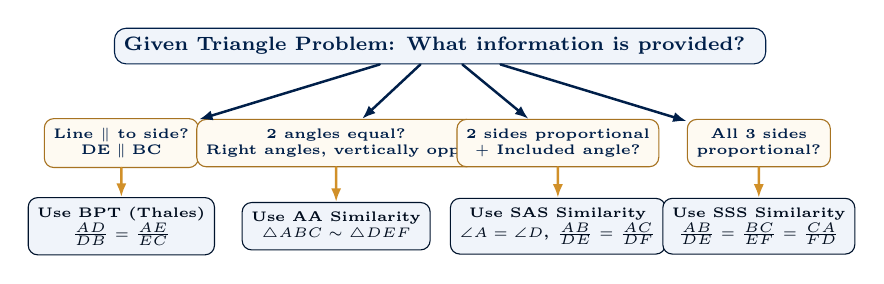
\begin{tikzpicture}[scale=0.88, line cap=round, line join=round]
  \node[draw=navy, fill=bluepale, rounded corners=1.5mm, font=\scriptsize\bfseries\color{navy}, align=center] (Start) at (0, 2.0) {
    Given Triangle Problem: What information is provided?
  };

  \node[draw=gold!80!black, fill=goldpale, rounded corners=1.2mm, font=\tiny\bfseries\color{navy}, align=center] (B1) at (-4.6, 0.6) {
    Line $\parallel$ to side?\\
    $\mathbf{DE \parallel BC}$
  };
  \node[draw=green!60!black, fill=greenpale, rounded corners=1.2mm, font=\tiny\bfseries\color{green!40!black}, align=center] (R1) at (-4.6, -0.6) {
    Use \textbf{BPT (Thales)}\\
    $\frac{AD}{DB} = \frac{AE}{EC}$
  };

  \node[draw=gold!80!black, fill=goldpale, rounded corners=1.2mm, font=\tiny\bfseries\color{navy}, align=center] (B2) at (-1.5, 0.6) {
    2 angles equal?\\
    Right angles, vertically opp.
  };
  \node[draw=green!60!black, fill=greenpale, rounded corners=1.2mm, font=\tiny\bfseries\color{green!40!black}, align=center] (R2) at (-1.5, -0.6) {
    Use \textbf{AA Similarity}\\
    $\triangle ABC \sim \triangle DEF$
  };

  \node[draw=gold!80!black, fill=goldpale, rounded corners=1.2mm, font=\tiny\bfseries\color{navy}, align=center] (B3) at (1.7, 0.6) {
    2 sides proportional\\
    $+$ \textbf{Included} angle?
  };
  \node[draw=green!60!black, fill=greenpale, rounded corners=1.2mm, font=\tiny\bfseries\color{green!40!black}, align=center] (R3) at (1.7, -0.6) {
    Use \textbf{SAS Similarity}\\
    $\angle A = \angle D$, $\frac{AB}{DE}=\frac{AC}{DF}$
  };

  \node[draw=gold!80!black, fill=goldpale, rounded corners=1.2mm, font=\tiny\bfseries\color{navy}, align=center] (B4) at (4.6, 0.6) {
    All 3 sides\\
    proportional?
  };
  \node[draw=green!60!black, fill=greenpale, rounded corners=1.2mm, font=\tiny\bfseries\color{green!40!black}, align=center] (R4) at (4.6, -0.6) {
    Use \textbf{SSS Similarity}\\
    $\frac{AB}{DE}=\frac{BC}{EF}=\frac{CA}{FD}$
  };

  \draw[-{Latex[scale=0.7]}, navy, line width=0.9pt] (Start) -- (B1);
  \draw[-{Latex[scale=0.7]}, navy, line width=0.9pt] (Start) -- (B2);
  \draw[-{Latex[scale=0.7]}, navy, line width=0.9pt] (Start) -- (B3);
  \draw[-{Latex[scale=0.7]}, navy, line width=0.9pt] (Start) -- (B4);

  \draw[-{Latex[scale=0.7]}, accent, line width=0.9pt] (B1) -- (R1);
  \draw[-{Latex[scale=0.7]}, accent, line width=0.9pt] (B2) -- (R2);
  \draw[-{Latex[scale=0.7]}, accent, line width=0.9pt] (B3) -- (R3);
  \draw[-{Latex[scale=0.7]}, accent, line width=0.9pt] (B4) -- (R4);
\end{tikzpicture}
\end{center}

\clearpage

% =============================================================================
% PAGE 12: BOARD EXAM TRAPS, VERIFICATION HACKS & PRE-SUBMISSION AUDIT
% =============================================================================
\thispagestyle{fancy}
\vspace*{0mm}

\chapterbanner{06}{EXAM TRAPS, HACKS \& PRE-SUBMISSION AUDIT}{Crucial Board Pitfalls, Instant Verification Checks \& Final Protocol}{\TrapTag}

\subhead{Module 12.1 $\vert$ Top 8 CBSE Board Exam Traps in Triangles}

\begin{enumerate}[label=\textbf{\color{navy}\arabic*.}, leftmargin=6.5mm, itemsep=1.8pt]
  \item \textbf{Vertex Order Mismatch in Similarity Statements:} Writing $\triangle ABC \sim \triangle DEF$ implies $\frac{AB}{DE} = \frac{BC}{EF} = \frac{CA}{FD}$. If you write $\triangle ABC \sim \triangle DFE$, your cross-multiplication will be mathematically invalid.
  \item \textbf{The Non-Included Angle Trap in SAS:} SAS requires the angle to be \textbf{between} the proportional sides. If $\frac{AB}{DE} = \frac{AC}{DF}$ and $\angle B = \angle E$, the triangles are NOT necessarily similar!
  \item \textbf{Applying BPT on Non-Parallel Lines:} You cannot apply $\frac{AD}{DB} = \frac{AE}{EC}$ unless $DE \parallel BC$ is explicitly given or proved first.
  \item \textbf{Confusing Segment Ratio with Whole Side Ratio in BPT:} BPT states $\frac{AD}{DB} = \frac{AE}{EC}$. Do not substitute $AB$ in place of $DB$ unless using the derived componendo form $\frac{AD}{AB} = \frac{AE}{AC}$.
  \item \textbf{Inverting Ratios in Trapezium Diagonals:} In trapezium $ABCD$, $\frac{AO}{OC} = \frac{BO}{OD}$. Students often mistakenly write $\frac{AO}{OC} = \frac{OD}{BO}$, reversing the transversal orientation.
  \item \textbf{Missing Theorem Statements in Proofs:} For BPT in subjective questions, you MUST write the formal \textit{"Given", "To Prove", "Construction"}, and state \textit{"triangles on same base between same parallels have equal areas"}.
  \item \textbf{Quoting Deleted Theorems:} Do not attempt to solve questions using the deleted Area Ratio Theorem ($\frac{\text{Area}_1}{\text{Area}_2} = k^2$). Stick to perimeter and linear side relations.
  \item \textbf{Unit Inconsistency in Shadow Questions:} Ensure shadow lengths and pole heights are in the same unit ($\text{m}$ or $\text{cm}$) before writing ratios.
\end{enumerate}

\subhead{Module 12.2 $\vert$ Arithmetic \& Geometric Verification Hacks}
\begin{itemize}[itemsep=1.2pt]
  \item \textbf{Cross-Multiplication Symmetry Check:} In $\frac{AD}{DB} = \frac{AE}{EC}$, check that $AD \cdot EC = DB \cdot AE$.
  \item \textbf{Scale Factor Consistency ($k$):} Compute $\frac{a_1}{a_2}, \frac{b_1}{b_2}, \frac{c_1}{c_2}$ separately; all three decimal quotients must be identical.
  \item \textbf{Positive Segment Filter:} For quadratic equations, reject any root that yields a negative length ($x - 2 < 0$).
\end{itemize}

\subhead{Module 12.3 $\vert$ The 5-Point Pre-Submission Board Exam Audit}

\begin{center}
\small
\begin{tabularx}{\textwidth}{>{\bfseries\color{navy}}c p{44mm} X}
\toprule
\rowcolor{bluepale}Check & Verification Item & Board Evaluation Standard \\
\midrule
$\square$ 1 & Vertex Correspondence Checked & Are the triangle vertices ordered so that corresponding angles match? \\
$\square$ 2 & Similarity Criterion Explicitly Stated & Did you write "(By AA similarity)" or "(By BPT)" next to every step? \\
$\square$ 3 & SAS Angle is Strictly Included & Is the equal angle located between the two proportional sides? \\
$\square$ 4 & Parallel Line Justification & Is the parallelism $DE \parallel BC$ clearly justified before invoking BPT? \\
$\square$ 5 & Final Units Explicitly Stated & Are units ($\text{cm}, \text{m}$) explicitly written after all length and shadow answers? \\
\bottomrule
\end{tabularx}
\end{center}

\vfill
\begin{center}
  {\color{gold}\rule{0.65\textwidth}{1.2pt}}\par\vspace{2mm}
  {\Large\bfseries\color{navy}Master the Theorems. Construct the Logic. Secure the 100\%.}\par\vspace{1.5mm}
  {\small\bfseries\color{gold}MATHS MANTHAN TUITION CLASSES}\par
  {\footnotesize\color{muted}contact@mathsmanthan.co.in \quad\textbar\quad +91-8171546558 \quad\textbar\quad \url{https://mathsmanthan.co.in}}
\end{center}

\end{document}
